\subsection{Opgave 37}

Figuren viser graferne for en lineær funktion g og et andengradspolynomium f.

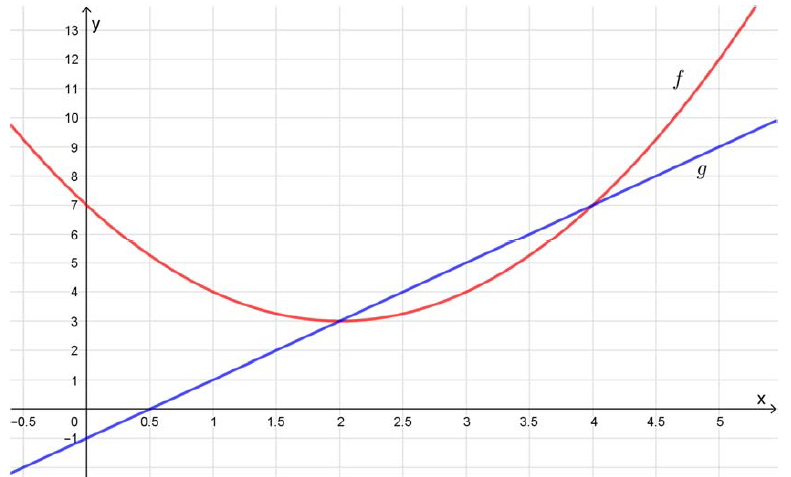
\includegraphics[width=8cm]{Opgave_31-40/Opgave_37/37.png}

Benyt figuren til at løse ligningen $g(x) = f(x)$.


\ans

For at løse ligningen $g(x) = f(x)$ skal vi altså finde de x værdier hvor y værdien for $g(x)$ og $f(x)$ er lig med hinanden.
Med andre ord skal vi finde x værdierne til de steder på grafen hvor $g(x)$ og $f(x)$ skærer hinanden.
Aflæser vi på grafen kan vi se at de skærer hinanden 2 steder ved x værdierne $x = 2$ og $x = 4$ hvilket er løsningen til ligningen $g(x) = f(x)$.
Skæringspunkterne er markerede på figuren nedenfor.

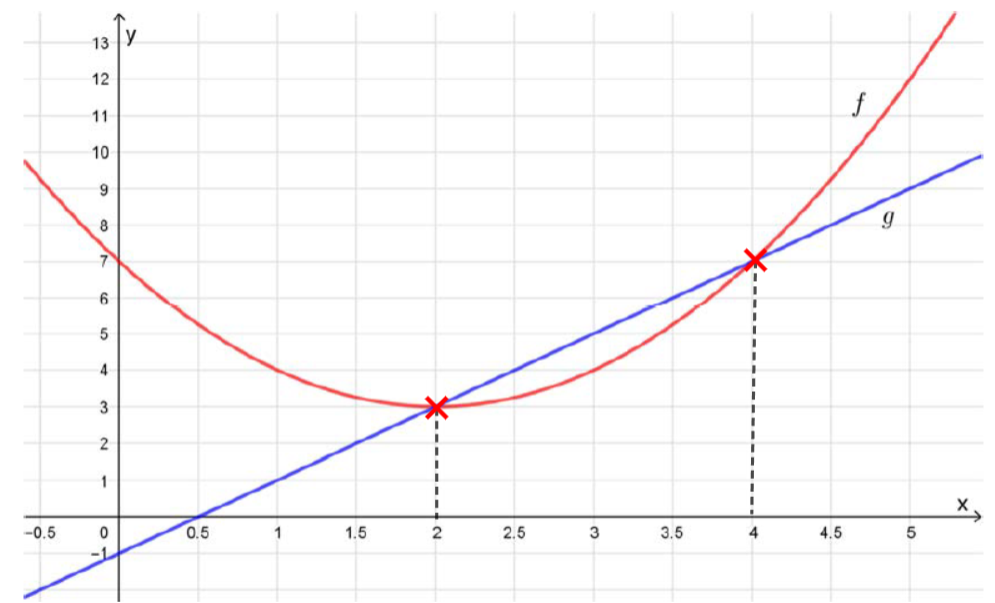
\includegraphics[width=8cm]{Opgave_31-40/Opgave_37/37.1.png}